\chapter{Provoz}
\label{ch:provoz}

Následující kapitola shrne možnosti realizovaného rozšíření pro koordinaci IoT, popíše, jaké je použití pro provoz
sítě internetu věcí a poté ověří realizované prostředky pro koordinaci IoT na produkčním příkladu.

\section{Nasazení a provoz systému}\label{sec:nasazení-a-provoz-systému}
Pro běh systému s realizovaným rozšířením bylo nutné zajistit následující prostředky:
\begin{itemize}
    \item \textbf{Server} \\
    Pro běh požadovaných komponent celého systému je požadován server, ke kterému budou schopny se uzly pomocí
    bezdrátové sítě připojit a bude schopen provozovat běhové prostředí Node.js -- v použitém příkladu se bude jednat
    o VPS s operačním systémem Debian ve verzi 9 \textit{skretch}.

    \item \textbf{Běhové prostředí pro nástroj Node-RED} \\
    Vzhledem k ekosystému nástroje Node-RED byl zvolen nástroj PM2\footnote{\url{http://pm2.keymetrics.io/}}, který pro
    aplikace v programovacím jazyce Javascript zajišťuje správu jejich běhu, tj. monitorování použitých systémových
    prostředků, jejich programové smyčky událostí či paralelní běh -- pro správce systému poskytuje možnost Node-RED
    spustit.

    \item \textbf{Broker MQTT} \\
    Jako broker byla zvolena implementace s názvem \emph{Eclipse Mosquitto}\footnote{\url{https://mosquitto.org/}} --
    jedná se o nástroj s otevřeným zdrojovým kódem od společnosti Eclipse.
    Broker dle dokumentace podporuje všechny z požadovaných vlastností (parametr zprávy \uv{retain}, tři úrovně QoS,
    zprávu poslední vůle atd.) a je dostupný jako aplikační balíček pro použitý operační systém.

    \item \textbf{Moduly ESP32} \\
    Pro produkční použití byly použity moduly ESP32 s deskou plošných spojů obsahující stabilizátor napětí, převodník
    UART-USB a lištu pinů umožňující zapojení do nepájivého pole -- jedná se o moduly s produktovým názvem
    \uv{ESP32-DevKitC}\footnote{\url{https://www.espressif.com/en/products/hardware/esp32-devkitc/overview}}
    přímo od firmy Espressif Systems.

    \item
\end{itemize}

Všechny výše uvedené prostředky jsem použil pro sestavení vlastního lokálního systému věcí.
\todo{vysledky mereni}
\missingfigure{Fotka z~nasazeneho systemu?}

\begin{figure}
    \centering
    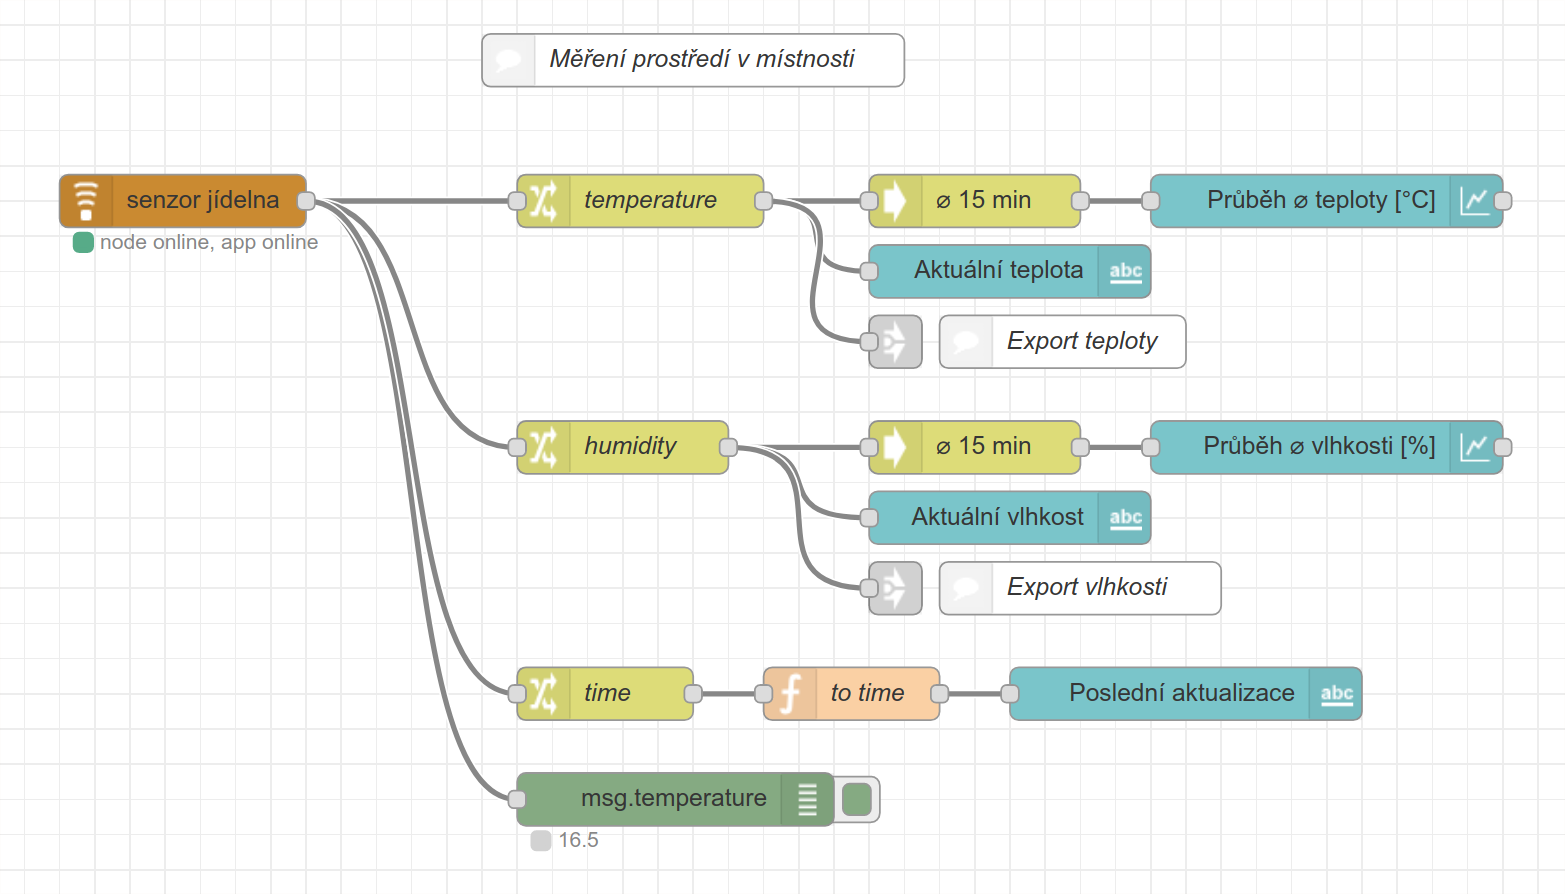
\includegraphics[width=\textwidth]{figures/fis-flow-1.png}
    \caption{Síť z produkčního nasazení nástroje Node-RED s realizovaných rozšířením -- TODO}
\end{figure}

\section{Produkční sítě}\label{sec:site-nástroje-node-red}
\missingfigure{screenshot z nasazene site}
